\chapter{Random Forest}
\section{Introduction}
Random forest, as the name suggests, is a classification method based on applying a group of decision trees. It belongs to classification methods which use simultaneous voting by more than one trained expert algorithm and the result is given by their majority (for regression tasks, by their average).

The random forest idea is based on an attempt to suppress over-fitting of (as well as correlation between) the trees in a group (forest). This suppression is achieved by randomly selecting attributes for each (sub)tree at each splitting node in addition to randomly selecting subsets of training samples using bagging (bootstrap aggregation); also refer to \cite{ref32,ref72}.

\subsection{Bootstrap}
Bootstrap is a statistical method based on random selection with replacement. This means that a 'set' created by this selection of samples may contain some examples multiple times (so, strictly speaking, it cannot be called a set).

The idea is that when some samples are randomly selected multiple times, some others are never selected - and those unselected samples may therefore be used as a test set.

The basic procedure is as follows. The data having $n$ samples are subjected to $n$ selections with replacement. The chance that an example will not be selected in any of $n$ attempts is based on that the probability of being chosen is $1 / n$ and inversely - of not being chosen, $1-1 / n$.

If the selection is repeated $n$ times, then multiplication of the probabilities provides the estimate of how many times no selection will be made:


\begin{equation*}
(1-1 / n)^{n}=e^{-1} \doteq 0.3678794412 \ldots(\text { for } n \rightarrow \infty) \tag{8.1}
\end{equation*}


For example, for 1000 selections with replacement, it is $(1-1 / 1000)^{1000}= 0.3676954248 \ldots \doteq 36.77 \%$.

Thus, there are two sets of samples now: $63.23 \%$ for training and $36.77 \%$ for testing, or, in other words, approximately $2 / 3$ for training and $1 / 3$ for testing. Sometimes this method is called ' 0.632 bootstrap.' Note that in this case, neither the training nor the testing set eventually contains multiplied samples.

The basic essence of classification by a forest of individually trained decisionmaking trees is shown in Figure 8.1. Defining the number of trees in a forest, $n$, and applying the bagging method to the original set of available training samples, $D$, a testing subset $d_{0}$ as well as a group of $n$ training subsets $d_{i}, 1 \leq i \leq n$, are generated, where $d_{i} \subset D, D=\cup_{i=0}^{n} d_{i}$.

Each of the $n$ trees is then trained using its own $d_{i}$ and works as a classifier. Because each of the trees in the created forest is usually more-or-less different

\begin{figure}[!ht]
\begin{center}
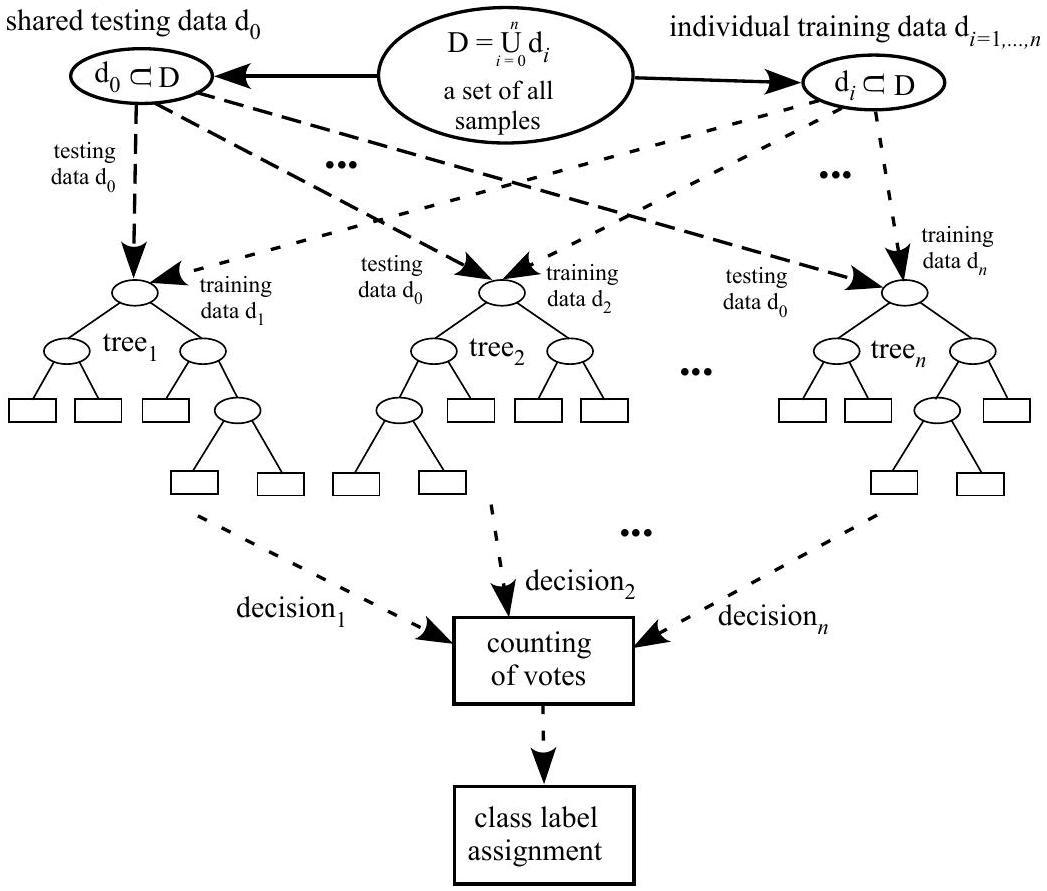
\includegraphics[width=0.9\textwidth]{chapter/Chapter8/2025_10_21_5ba6420d88ee7388cb5eg-209.jpg}
\caption{Random trees - the main idea of a classifier group composed of $n$ decision trees that are trained by randomly selected subsets of training samples.}
\end{center}
\end{figure}

from the rest, it is quite possible that their classification of a given unlabeled item differs as well - the reason is the fact that those trees are based on more-or-less different subsets of attributes. As a result, the relevance of the same attributes may be quite different for each tree. The resulting assignment of the class label to the classified item is finally determined by the prevailing majority in the vote.

And the final question: What is the best number $n$ of trees? The optimal number is achieved when adding more trees does not improve the classification. This value can be found experimentally for practical applications - direct determination is generally not supported by theory. Two requirements should be met: the lowest classification error and the smallest number of trees.

\subsection{Stability and Robustness}
In order to avoid 'too good' or 'too bad' a random selection (which is also quite possible), it is advisable to repeat experiments, each time with a different seed of the (pseudo)random number generator (better still, is to use a real random number source, which may not always be achievable).

In general, each testing can provide a more or less different estimated future classification error, so the expected error value is calculated as the average (it also applies to cross-validation). The variance of the average expected error provides information on the stability of the algorithm with respect to data composition. To achieve good stability (algorithm robustness), the smallest possible variance is ideal.

This mainly affects the data itself, but different algorithms can give different results from the same point of view, though the average error may be almost the same. The test results are therefore another aspect of the algorithm selection and robustness, which is a fundamental truth for decision trees that can very easily suffer from instability due to even small changes in training examples.

\subsection{Which Tree Algorithm?}
In principle, what kind of decision tree is used is not decisive. Often, implementations and software packages with CART (Classification And Regression Tree; for details see \cite{ref36}) are used, but $c 5$ or others could be employed as well. For practical reasons and simplicity, the CART system is used in the following demonstration because it is easily available in R .

\section{Random Forest in R}
This chapter presents a brief demonstration of applying the random forest method in R to the same sample of data as in the previous cases (the reviews of books). The demonstrated use of the random forest method here, based on a popular R-\\[0pt]
package randomForest, comes from the original implementation in the Fortran programming language by statistician Leo Breiman (January 27, 1928 - July 5, 2005). For more details, see \cite{ref33,ref34,ref35}. The detailed description of randomForest parameters in R can be found in \cite{ref171}.

\begin{verbatim}
library(randomForest)
# loading the data
data <- read.csv("BookReviews.csv", header=TRUE)
# converting the data to a matrix
dtm <- as.matrix(data)
# removing the object data (unnecessary from now)
rm(data)
# number of instances
n <- dim(dtm)[1]
# number of attributes
m <- dim(dtm)[2]
# indexes of 100 testing samples
number_of_test_samples <- 100
test_index <- 1:number_of_test_samples
# selecting training samples
train_data <- dtm[-test_index, 1:(m-1)]
train_labels <- dtm[-test_index, m]
# selecting testing samples
test_data <- dtm[test_index, 1:(m-1)]
test_labels <- dtm[test_index, m]
# training a random forest model
rf_model <- randomForest(train_data, as.factor(train_labels))
predictions <- predict(rf_model, test_data, type="response")
# creating a confusion matrix
cm <- table(test_labels, predictions)
print("Confusion matrix")
print(cm)
\end{verbatim}

\begin{verbatim}
# number of instances
n <- sum(cm)
# number of correctly classified instances for each class
correct <- diag(cm)
# numbers of instances in each class
instances_in_classes <- apply(cm, 1, sum)
# numbers of each class predictions
class_predictions <- apply(cm, 2, sum)
# accuracy
accuracy <- sum(correct)/n
# precision per class
precision <- correct/class_predictions
# recall per class
recall <- correct/instances_in_classes
# F1-measure per class
f1 <- 2 * precision * recall / (precision + recall)
# printing summary information for all classes
df <- data.frame(precision, recall, f1)
print("Detailed classification metrics")
print(df)
print(paste("Accuracy:", accuracy))
# macroaveraging
print("Macro-averaged metrics")
print(colMeans(df))
# microaveraging
print("Micro-averaged metrics")
print(apply(df, 2, function (x)
    weighted.mean(x, w=instances_in_classes)))
# plotting the error rates or MSE of the randomForest object
plot(rf_model, col=c(1,2,4), lwd=1.5, lty=1)
rf_legend <- if (is.null(rf_model$test$err.rate)) {
    colnames(rf_model$err.rate)
\end{verbatim}

\begin{verbatim}
            } else {
                colnames(rf_model$test$err.rate)
            }
legend("topright", cex=1, legend=rf_legend, lty=1,
    col=c(1,2,4), horiz=TRUE)
\end{verbatim}

As a result, the script returns the following output:

[1] "Confusion matrix"
\begin{flushleft}
\begin{tabular}{lll}
test\_labels & 0 & 1 \\
0 & 38 & 10 \\
1 & 9 & 43 \\
\end{tabular}
\end{flushleft}

\begin{verbatim}
[1] "Detailed classification metrics"
precision recall f1
00.80851060 .79166670 .8000000
10.81132080 .82692310 .8190476
[1] "Accuracy: 0.81"
[1] "Macro-averaged metrics"
precision recall f1
0.80991570 .80929490 .8095238
[1] "Micro-averaged metrics"
\end{verbatim}

\begin{flushleft}
\begin{tabular}{rrr}
precision & recall & f1 \\
0.8099719 & 0.8100000 & 0.8099048 \\
\end{tabular}
\end{flushleft}

The graph in Figure 8.2 shows the classification accuracy error dependence on the number of trees in the random forest. The graph contains curves for the positive class (marked as 1 ), negative class (marked as 0 ), and the OOB (Out-OfBag, the standard mean error for both classes measured using the test samples).

As a reader can see, the classification accuracy is better than $80 \%$. For a small number of random trees, the classification error is relatively high, especially at the beginning: for just one random tree, the error is nearly $50 \%$, which corresponds to a random guess. With the increase in forest size, the error decreases, very quickly initially. After reaching a certain number of trees, around the vicinity of 300 , the classification no longer improves. Thus, 300 random trees is perhaps the optimal solution.

Such a number of trees might look very high - however, each tree is generated by a limited number of attributes (words) because it uses only a relatively small subset of all training samples, therefore a limited vocabulary. As a result, each tree is also relatively small, perhaps not a very 'smart' expert but nonetheless, a real expert in its narrow area.

\begin{figure}[!ht]
\centering
  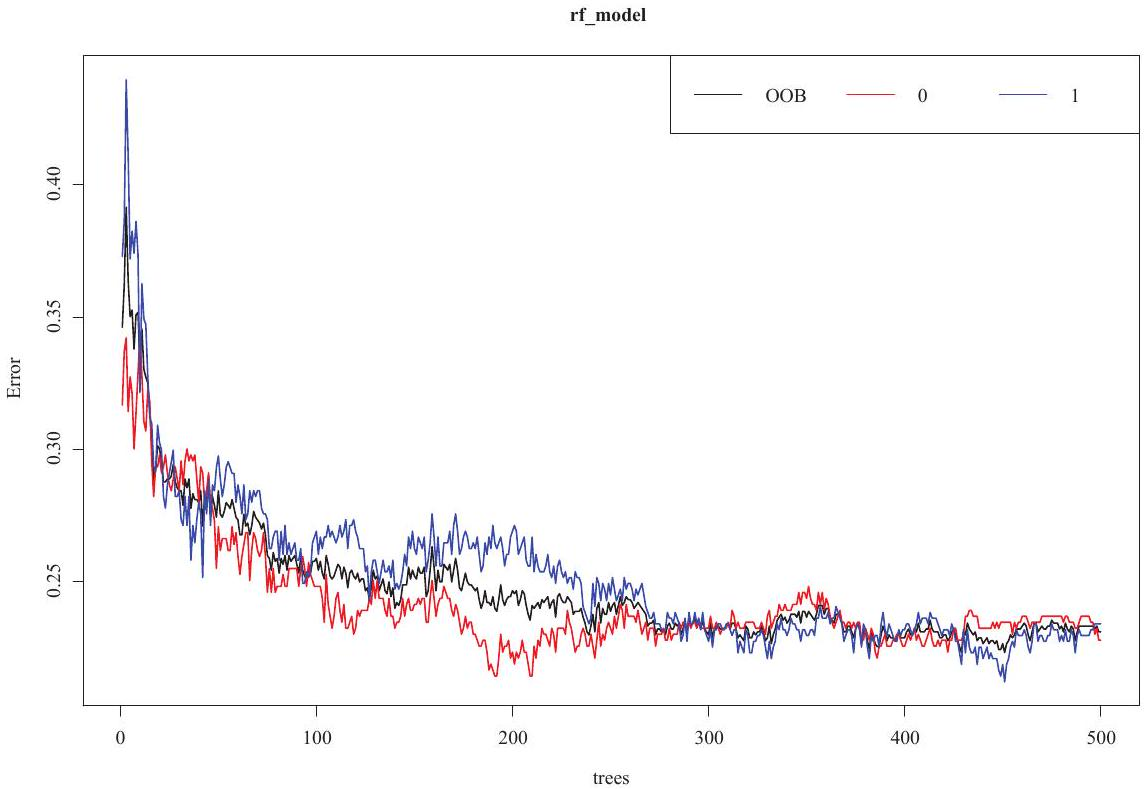
\includegraphics[width=0.5\textwidth]{chapter/Chapter8/2025_10_21_5ba6420d88ee7388cb5eg-214.jpg}
\caption{Classification accuracy dependence on the number of trees (around 200 trees, OOB is in the middle, 0 bottom, 1 top).}
\end{figure}

However, very good results can be achieved by gathering limited experts whose areas somehow overlap with each other, which is one of the main and successful ideas of the method used and presented here. In recent times, the popularity of random forests in many practical application areas has shown an increase.\\